\documentclass{scu-thesis}
% \usepackage{graphicx}	% for including graphics
% \usepackage{amsmath}	% for advanced typesetting of mathematics
% \usepackage{txfonts}	% for using the Times-Roman font
% \usepackage{natbib}	% for better citation styles

\usepackage[letterpaper, portrait, margin=1in]
{geometry}

\geometry{	
lmargin = 1.25in,
rmargin = 1.25in,
}

\usepackage{graphicx}
\graphicspath{ {images/}}


% These must be set first ... the rest of the thesis commands rely on them.

\author{Eric Beckmann}
\author{Jonathan Coon}
\author{Mikael Figueroa}
\author{Matthew Voss}
\title{Crowdify}
\department{Department of Computer Science and Engineering}
\degree{Bachelor of Science in Computer Science and Engineering}

% Only bachelor's theses should have multiple authors and/or be from
% multiple departments.  Signatures required:
%
% Bachelor's theses: advisor(s), department chair(s)
% Master's theses: advisor, reader, department chair
% Doctoral theses: doctoral committee (including advisor), department chair

\begin{document}
\frontmatter
\signature{Thesis Advisor}
\signature{Thesis Advisor}
\signature{Department Chair}
\signature{Department Chair}

\maketitle
\begin{abstract}
Backup systems are an important part of any IT infrastrucutre. They provide data assurance in the face of faulty hardware and software. Nonetheless, computer users commonly rely on backup systems that fail to exhibit either reliability, accessibility, security, or a combination of all three. We work to resolve this issue by creating a storage system in which users share encrypted data fragments amongst each other instead of with a single data storage entity. If data is corrupted on any single storage device, the data may be restored from a set of other storage devices.  Furthermore, this data is dispersed geographically. These architectural features of the sytem provide greater reliability and accessibility while the lack of any central service provider allows users to retain ownership of their data, improving privacy.
\end{abstract}


\tableofcontents
\listoffigures

\mainmatter
\chapter{Introduction}
Data loss is a fundamental, widespread problem in computing. In a single year, 25\% of PC users will lose their data. Furthermore, 100\% of all data storage technologies, ranging from magnetic tapes to hard drives to solid state storage, will inevitably fail. \footnotetext[1]{http://www.imagineiti.com/backup/biggest-backup-mistake/} Data loss is not only unavoidable, it is potentially devastating. 70\% of small businesses that experience major data loss go out of business in a year.\footnotemark[1] Moreover, the U.S. loses an estimated \$18.2 Billion every year due to data loss. \footnotetext[2]{https://gbr.pepperdine.edu/2010/08/the-cost-of-lost-data/} Almost every industry relies on accurately storing and accessing information, whether this be in the form of financial archives, software developmental codes, customer data, order records, etc. Backups, which are systems for duplicating one’s data and storing it in another place, counteract data loss.


\section{Motivation}
Many current solutions implement data backup. We observe, however, that all systems suffer problems with privacy, accessibility, resilience, or a combination of all three. Two general categories describe current solutions: enterprise backup, cloud backup and personal backup. Unfortunately, current enterprise solutions cannot be examined as they are often highly customized and proprietary. Cloud backup is a service in which users upload files to be stored in a data center. These systems, while they are highly redundant, are not immune to corporate problems. If the company providing your backups goes out of business, your backups will no long be accessible. In addition, these services may go down from time to time. Amazon S3, a common back end for such systems, has been known to have long outages \footnotetext[3]{https://gigaom.com/2008/07/20/amazon-s3-outage-july-2008/} \footnotetext[4]{http://www.rightscale.com/blog/cloud-industry-insights/amazon-ec2-outage-summary-and-lessons-learned/}. Personal backup, on the other hand, is the solution used by diligent individuals who regularly save their files to an external storage device or media. While personal backup addresses the privacy issue, the system is not resilient, since the external storage device will lose all the backup data if it ever fails \footnotetext[5]{https://www.backblaze.com/blog/hard-drive-reliability-stats-for-q2-2015/}. In addition, accessibility to the data relies on constant access to a single device.

\section{Solution}
Our backup system will address the issues of privacy, accessibility, and resilience. It will use redundancy and wide geographic distribution to create greater resiliency. We imagine at least one storage system per network. These storage systems will be interconnected, allowing them to share data. The data will be distributed as widely as the networks using these devices, encouraging hardware redundancy and making sure the data is constantly accessible. The protocol, once designed will be frozen, ensuring that these systems will continue to provide their services, even if support is no longer possible. Regarding privacy, we will not have access to the users' data, and each user's data will be only be accessible by the user who owns the data through encryption as mentioned above.

\chapter{Activity Diagram}

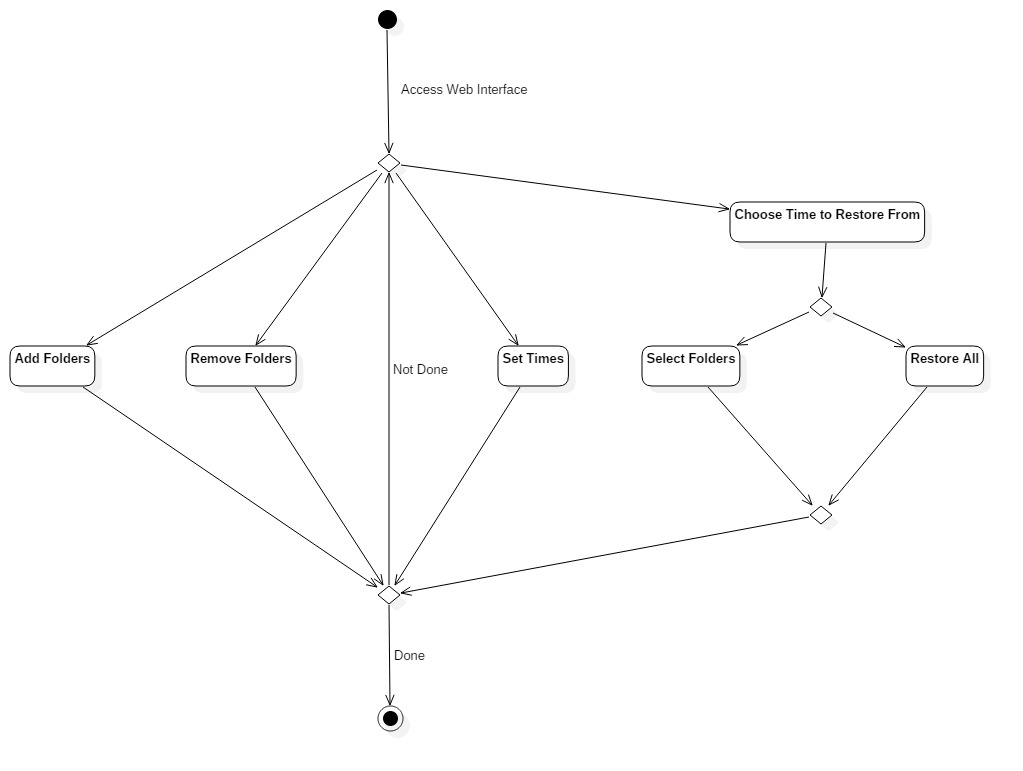
\includegraphics[scale=0.45]{images/ActivityDiagram1.jpg}
\chapter{Testing Plan}

The purpose of this system is to provide a secure, private, efficient, reliable, and constantly accessible data backup system.  Therefore, any failures could be critical, possibly causing people or corporations to lose their data and resulting in millions of dollars in damages.  It is our responsibility to ensure that each individual component of the system works perfectly, and also that the system as a whole smoothly functions.

Since our intended system is very complex and consists of several modules, we will most likely follow an incremental process model, and use the continuous integration approach.  Under this method, performing unit testing is very intuitive, as each team member will continuously test their own modules in isolation as they develop them.  We will remember to test early and often in order to catch bugs as soon as possible.  Part of this will be white box testing for code coverage; at the very least, we should make sure all  linearly independent paths through the code are tested.  Furthermore, we will make careful documentation of all bugs we catch.  This practice will help us get a better idea of common failure points in our modules, so we can focus more on those areas when we test later on.  At least once per month, we will peer-review each others' modules in order to ensure good coding practices, including high cohesion and low coupling.  Once we have a working system, we will perform black box testing with team members using the system for their own personal backups, and sharing files amongst the four of us.

Besides testing within the team, we should also open testing up to focus groups representing hypothetical users.  Once our system reaches a fully-working version, we will find friends and family members to try using our system.  The obvious problem is that we cannot ask them to rely fully on our system as a replacement to the backup systems they already use, because if our system fails that will represent a great inconvenience and loss to them.  Therefore, we will ask them to use our system in addition to whatever backups they currently use.  Our final system relies on a large network of users sharing files with each other using a peer-to-peer protocol; therefore at some point we should open the system up to the general public for beta testing.  Once again, we must put a disclaimer as clearly as possible that this system cannot yet guarantee privacy and reliability.  A public beta testing would definitely require the most effort to implement and maintain, but it will be necessary before we can release any type of product.  We may not reach this phase in the course of this year, but if we continue the project later we definitely will.
\chapter{Societal Issues}

\section{Ethical Discussion, Social Concerns, and Compassion}

\subsection{Justification}
	There are many ethical justifications for our project.  In the larger sense, we hope to make the world a better place by providing a better data backup and restore service than what is currently out there.  The bottom line is that our product will provide a convenience to the general public and assist them with storing files and also protecting against the problems of data loss.  Specifically we will help corporations become more efficient in their operations, which could bring economic prosperity and higher standards of living for society as a whole.  This is all in agreement with the first rule of the ACM Code of Ethics to ''contribute to society and human well-being.'' \cite{acmethics}

	Our project also deals directly with the human right to privacy.  As detailed in rule 1.7 of the ACM code of ethics, we are to ''respect the privacy of others.'' \cite{acmethics}  Furthermore, privacy is listed as a fundamental human right in Article 12 of the Universal Declaration in Human Rights: ''no one shall be subjected to arbitrary interference with his privacy.'' \cite{udhr}  The right to privacy is an inalienable human dignity that we hope to protect.  Privacy is so important because it gives people greater freedom to make their own moral decisions, independent from the judgement of others and shielded from the pressure to conform to their culture.  As one adage goes: ''The time you spend alone with yourself is the most precious time you have.  This is your proving ground.  It’s where you decide who you are, what values you uphold, and ultimately how you are seen in the eyes of yourself and others.'' \cite{wolf}

	The right to privacy is especially pertinent in this day and age, where more and more of everyone’s personal data is being put out online, vulnerable to access by malicious parties.  We hope our service will allow people to protect their privacy, since instead of storing their data in a single corporation’s database, which presupposes full trust in that corporation, and also provides a single point of attack for governments or hackers who wish to seize the data, we will be distributing the encrypted data securely to many locations in separate fragments.  These are not merely hypothetical concerns.  Data stores run by single entities have suffered data breaches many times in the past.  For example, Apple iCloud was hacked in August of 2014, which resulted in many celebrity photographs being leaked. \cite{independent}  Furthermore, the NSA has controversially forced companies like Google and Yahoo to turn over customer data in moves that have widely been called unconstitutional. \cite{gizmodo}  Our system will not be vulnerable to privacy violations like this, because there will no longer be a single party attackers can go after to view people's data.

\subsection{Lifelong Learning}

	Throughout this project, it is also very important that we are mindful of our own growth in moral character and technical skill.  Our society is increasingly dependent on computers, so as computer engineers we have a large role for improving people’s daily lives.  As we go through this project, we will be sure to adhere to the Software Engineering code of ethics.  We will make every effort to put the public interests and the common good first.  We will strive for the highest quality work in all aspects.  We will strive to cultivate our own character, skills, and abilities, and will seek to grow as much as possible through this project.  Finally, we will treat each other with respect during this project.

\subsection{Possible Pitfalls}
	As with most engineering projects, there are certain moral pitfalls that we might encounter along the way.  First of all, we have to consider that potential users of our system are trusting us to keep their data as private as possible.  If we take any shortcuts or make any oversights while designing our system, we could leave security holes that will compromise privacy.  By not keeping people's data private, we expose them to malicious parties such as idenity thieves, hackers, fraud artists, and so on.  We would be indirectly responsible for any damage caused, because we made people believe they had privacy which they did not.  And this would break article 1.7 of the ACM Code of Ethics to ''Avoid harm to others''. \cite{acmethics}  It is therefore our duty to ensure privacy in our system to the maximum extent possible.

	There is also the possible pitfall of our system being used by criminals, due to the enhanced privacy it provides.  By providing a system by which users can store their data with complete privacy, we could allow criminals to hide evidence of their activities, obstructing the activities of legitimate law enforcement agencies. The peer-to-peer architecture we use is similar to protocols such as BitTorrent which are far and wide used only for illicit purposes.  Even though it is not our intention that our system would be used for illegal activities, we must consider this possibility.

\section{Political Concerns}
	This is not a public project, so we can mostly disregard political concerns.

\section{Economic considerations and Manufacturability}
	The scope of the project at this stage is not to deploy a large scale product for the public to use, but rather to make a system for the purposes of testing new algorithms and methods of data distribution.  Therefore, we will not consider the costs of deploying a final product at this time.

	As for the costs of prototyping itself, we expect it to be quite low.  The software development costs little to no resources.  We will use a number of Raspberry Pi boards to implement our system.  At the cost of \$40 per board, we expect the total cost of the project to be no more than \$300.  We will support this project with our own personal funds.

\section{Health and Safety}
	This project does not require the use of any heavy machinery, extraordinarily large power sources, etc.  Therefore, we don't need any special safety considerations for this project.  However, we will be using electronic equipment such as PCs and Raspberry Pis in the course of this project, so we should exercise common sense as we would handling any electronic appliance.

\section{Sustainability and Environmental Impact}
	The environmental impact of creating our starting system should be minimal, since it is quite small scale and only uses a few electronic devices.  For the reasons mentioned above we will not yet consider the costs of deployment for a large scale system.

\section{Usability}
	One of the requirements and goals for our system is to make our interface as user-friendly as possible.  We will do this by only providing our user with a basic set of controls, hiding the complexity of the data distribution algorithm from them.  It is also important that our system be easy to set up as well.  We can acheive this by making a good installer as well as utilizing auto-configuration to the fullest extent.  Finally, we will do our utmost to prevent hogging of system resources by our program, so that it runs as transparently in the background as possible.

\bibliography{master}
\bibliographystyle{ieee}

\backmatter
\end{document}